\chapter{Proposed Solution}

%As stated by Sadana et al. \cite{sadana_redefining_2016}, it is also important to explore how existing techniques can be applied to new platforms like virtual reality devices.
%We got inspired by a circular form of a tree map plot for hierarchical structures (see Figure \ref{fig:hierarchicalCirclePlot}). Each node can either be a simple leaf node or a network itself. So we need a way to visualize connections between different networks, a way to do this is a multilayer network visualization see Figure \ref{fig:2dmultilayerVis}. Here each flat layer represents a different network but a hierarchical relationship is not always given for these visualizations.  
\section{Initial Problem}

The idea to build our own visualization began as we wanted to improve the original visualization of the comorbidity network we saw in Figure \ref{fig:original2DdiseaseNet}. Data analysts use this and similar datasets to discover possible coherences, correlations, distributions, clusters and more in the data. 
However, the visualization was not optimal because it hides links and first and foremost is limited to only one hierarchical layer. This is not a problem for this dataset in particular, but we wanted a solution to visualize n hierarchical networks.\\
Therefore, our goal is to develop a new visualization tool which supports data analysts in their daily work analyzing hierarchical networks, with the comorbidity network as a first real world data example. To test the usability of the visualization for n hierarchical networks we created some randomized networks as test data. 

\section{Main concept}

\subsection{Layout}

\begin{figure}[h]
    \centering
    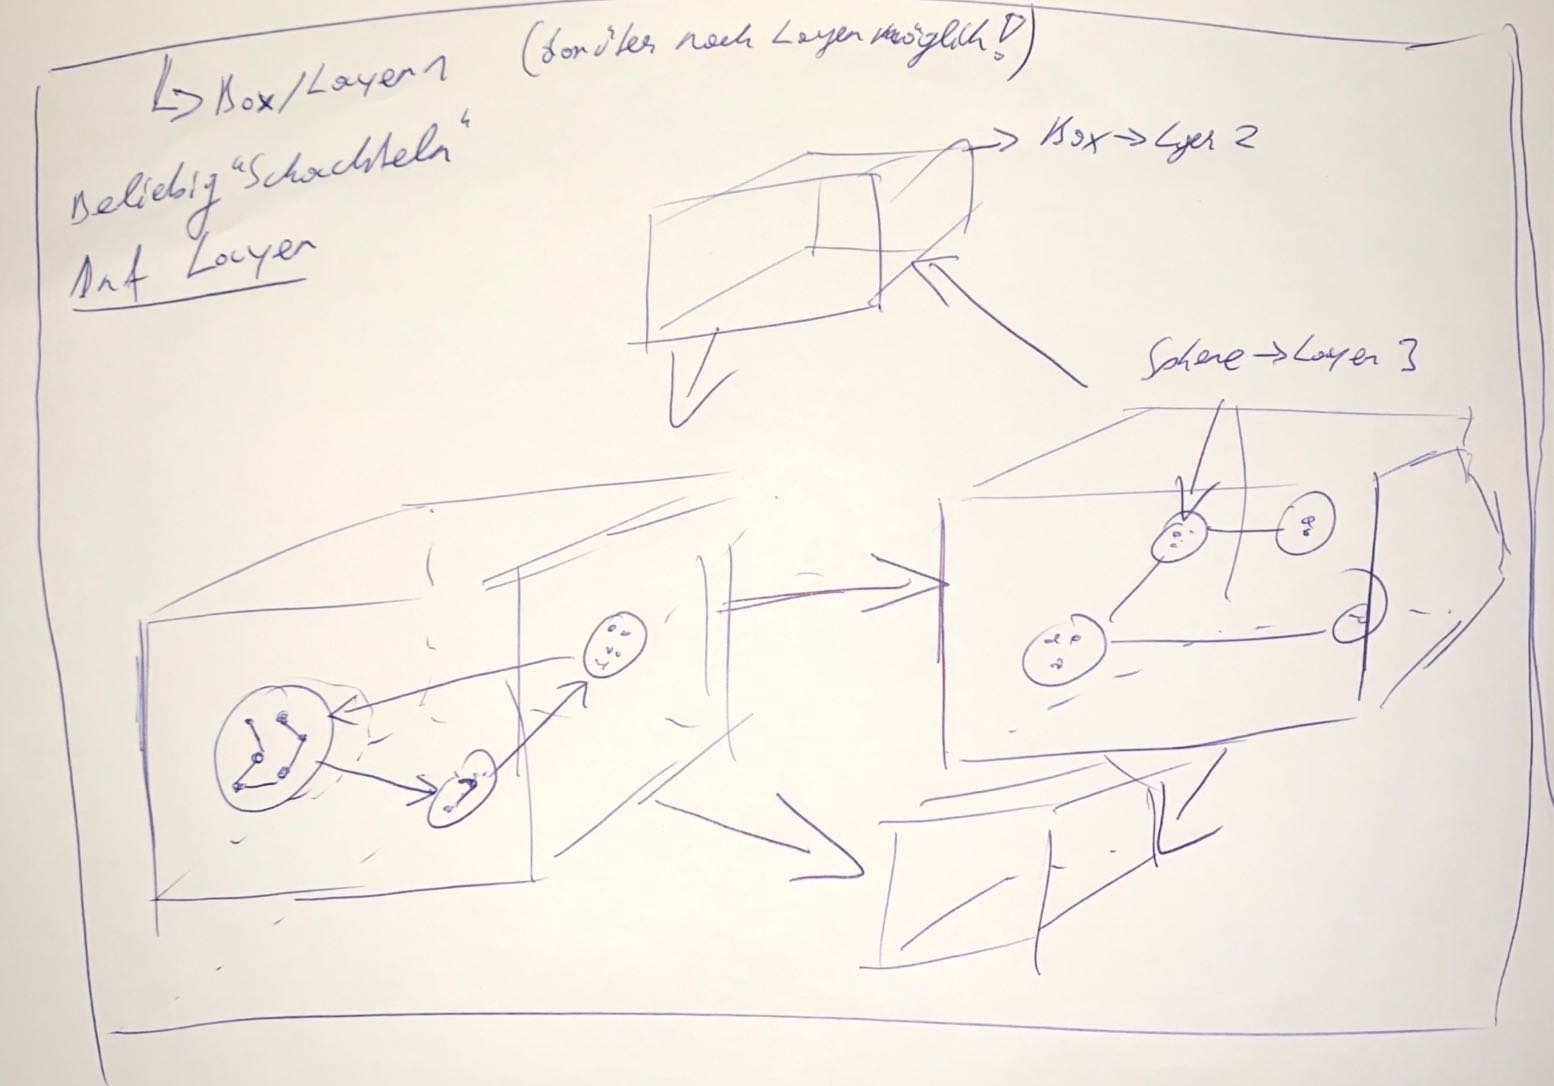
\includegraphics[width=1\textwidth]{chapters/graphics/concept1.jpg}
    \caption{(TODO redraw sketch)A sketch of our preferred layout. } 
    \label{fig:layoutSketch} 
\end{figure}

Verbindung zwischen Datenstruktur und Layout\\
Ziel des Layouts und Begründung (flexbilität, Kombination standard force based und hierarical/constraint based)\\
Liste an Forces\\
Prozess Optimierung der Forces (nacheinander wirken, Sicherheitspuffer)\\
Wichtigkeit Zusammenhang der Forces mit dem Renderprozess, Stichwort Node Größe

\subsection{Render Visuals}

Transparente Nodes\\
Node Label + weighted Link\\
different Colors for links\\
Ausblenden des Nodes wenn innerhalb, innersten Node mit Wireframe anzeigen => verbessert Übersichtlichkeit\\

\subsubsection{Exploration Flow}

Grundsätzliche Idee wie die Daten analyisert werden\\
Overview am Beginn => außenansicht \\
Wechsel zur Detailansicht\\
Möglichkeit von Room scale voll ausschöpfen, walk around the vis\\
Verschiedene Filteroptionen für Edges (nur grundidee)\\
Verschiedene Navigationsmethoden (nur grundidee)\\

\section{Navigation + Interaction}

Laserpointer Interaktion zum selektieren von Nodes / links\\
Navigations Methoden\\
Anzeige des currentLayers am Controller\\
Grafik mit Controller button belegung\\

\section{Challenges}

Visual Clutter: Filtermethoden von links (2 separated methods)\\

Problem Größenbezug real world + virtual scene\\
1. Dynamischen fly speed\\
2. Dynamisches skalieren\\
manueller speed + skalierung wichtig da nicht klar was User preferred und wie groß sein space ist\\ 


\section{(eventuell) Alternative Concepts}

verworfene Konzepte, 2 Layer Concept\\

\chapter{old - Proposed Solution}
Ideas:
\begin{itemize}
    \item Progress
        \begin{itemize}
            \item begin flat multilayer rendering
        \end{itemize}
\end{itemize}

\section{Concepts}
\subsection{Original 2D Visualization}
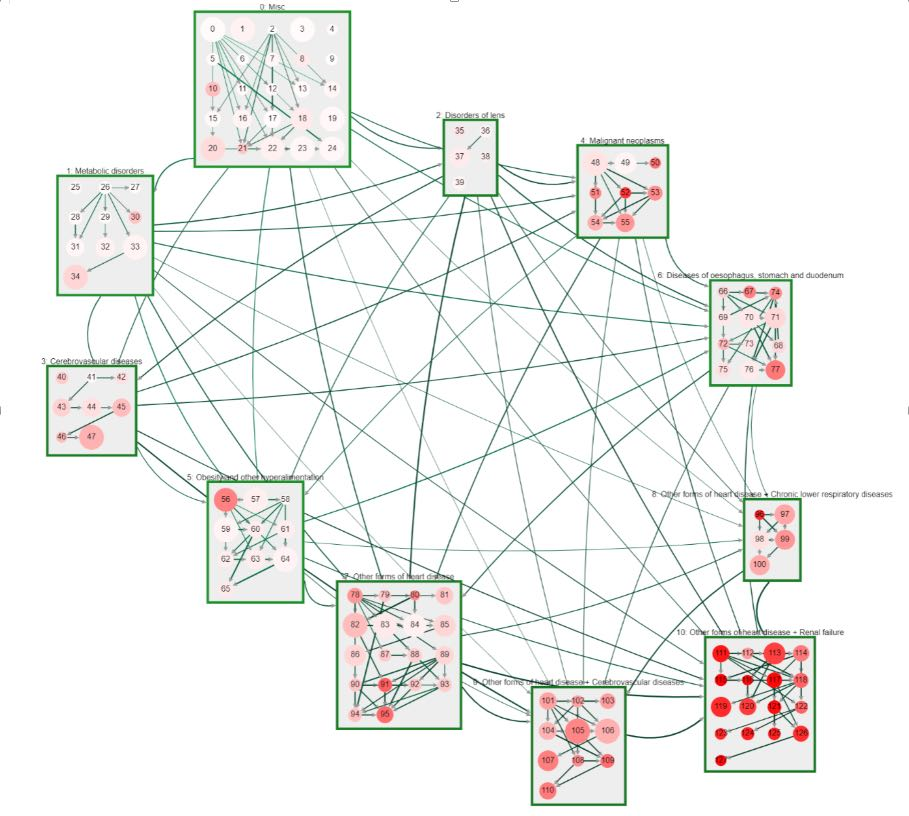
\includegraphics[width=0.5\textwidth]{chapters/graphics/2dVisOfDemoData.jpg}

Problem only two layers supported

\subsection{2-Layer Concept}
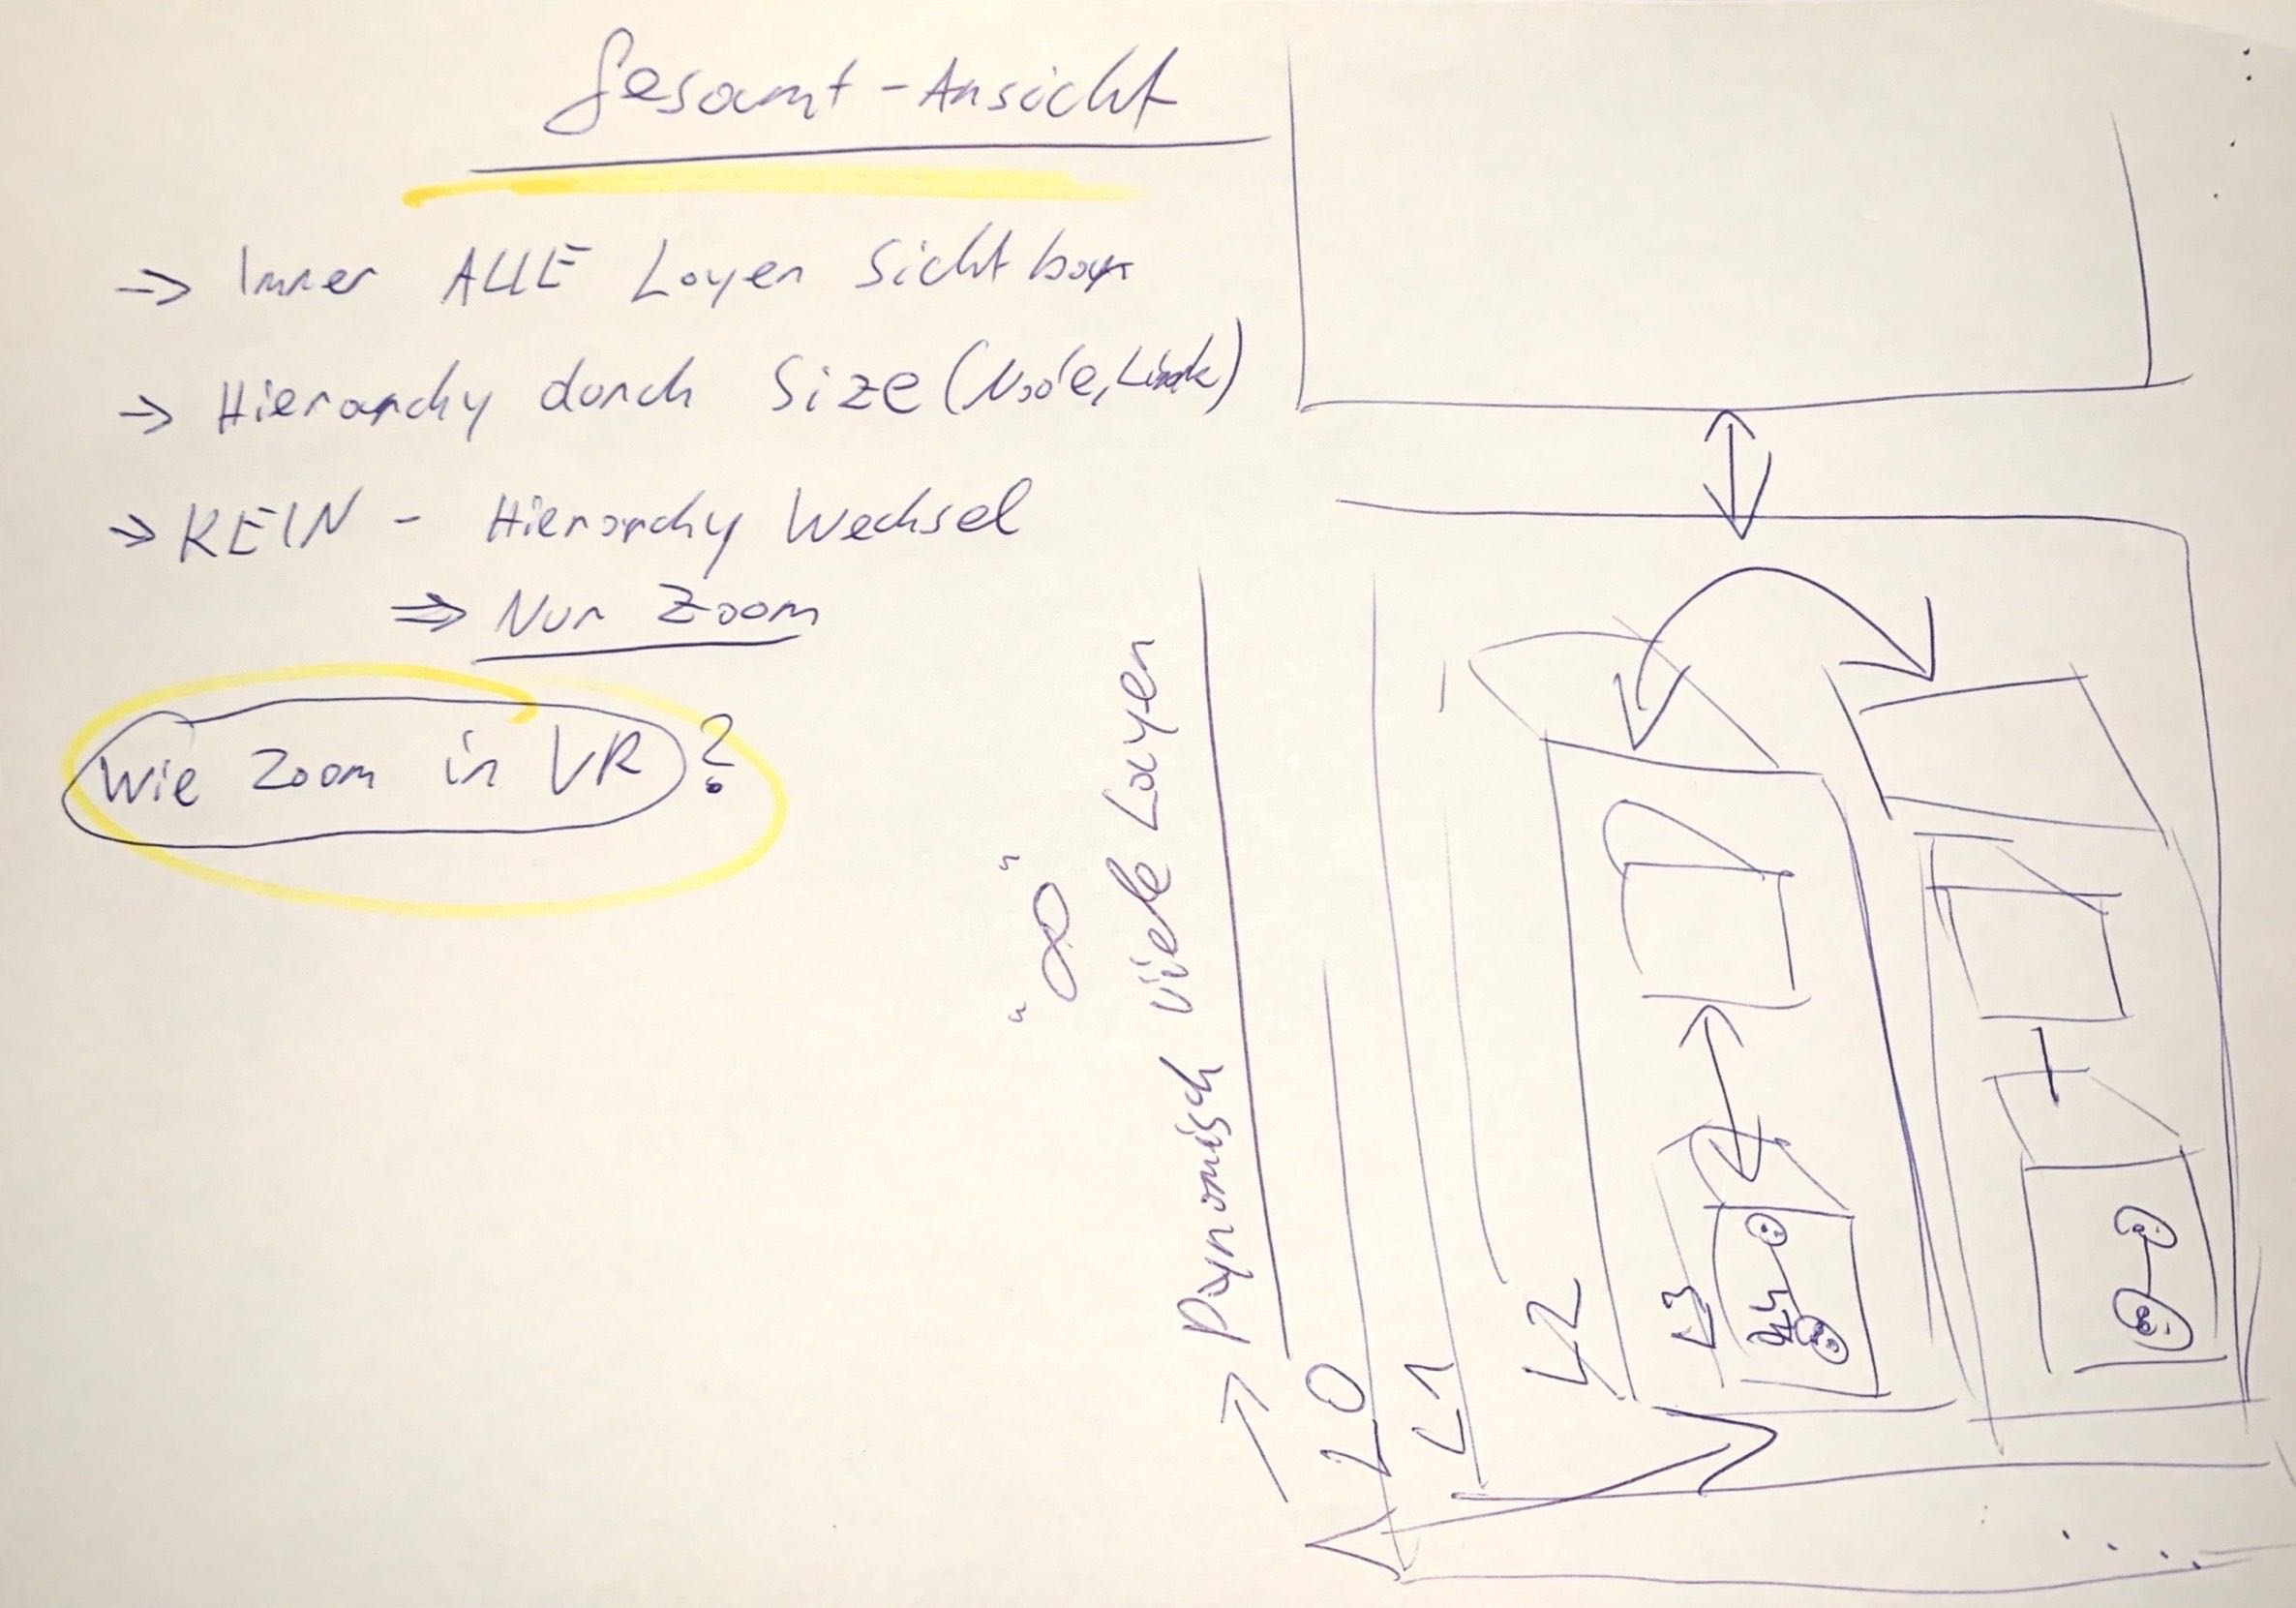
\includegraphics[width=0.5\textwidth]{chapters/graphics/concept2.jpg}

Cube/ (half) sphere position of sub-graphs \\
Starting idea, why it was discarded

\subsection{n-Layer Concept}
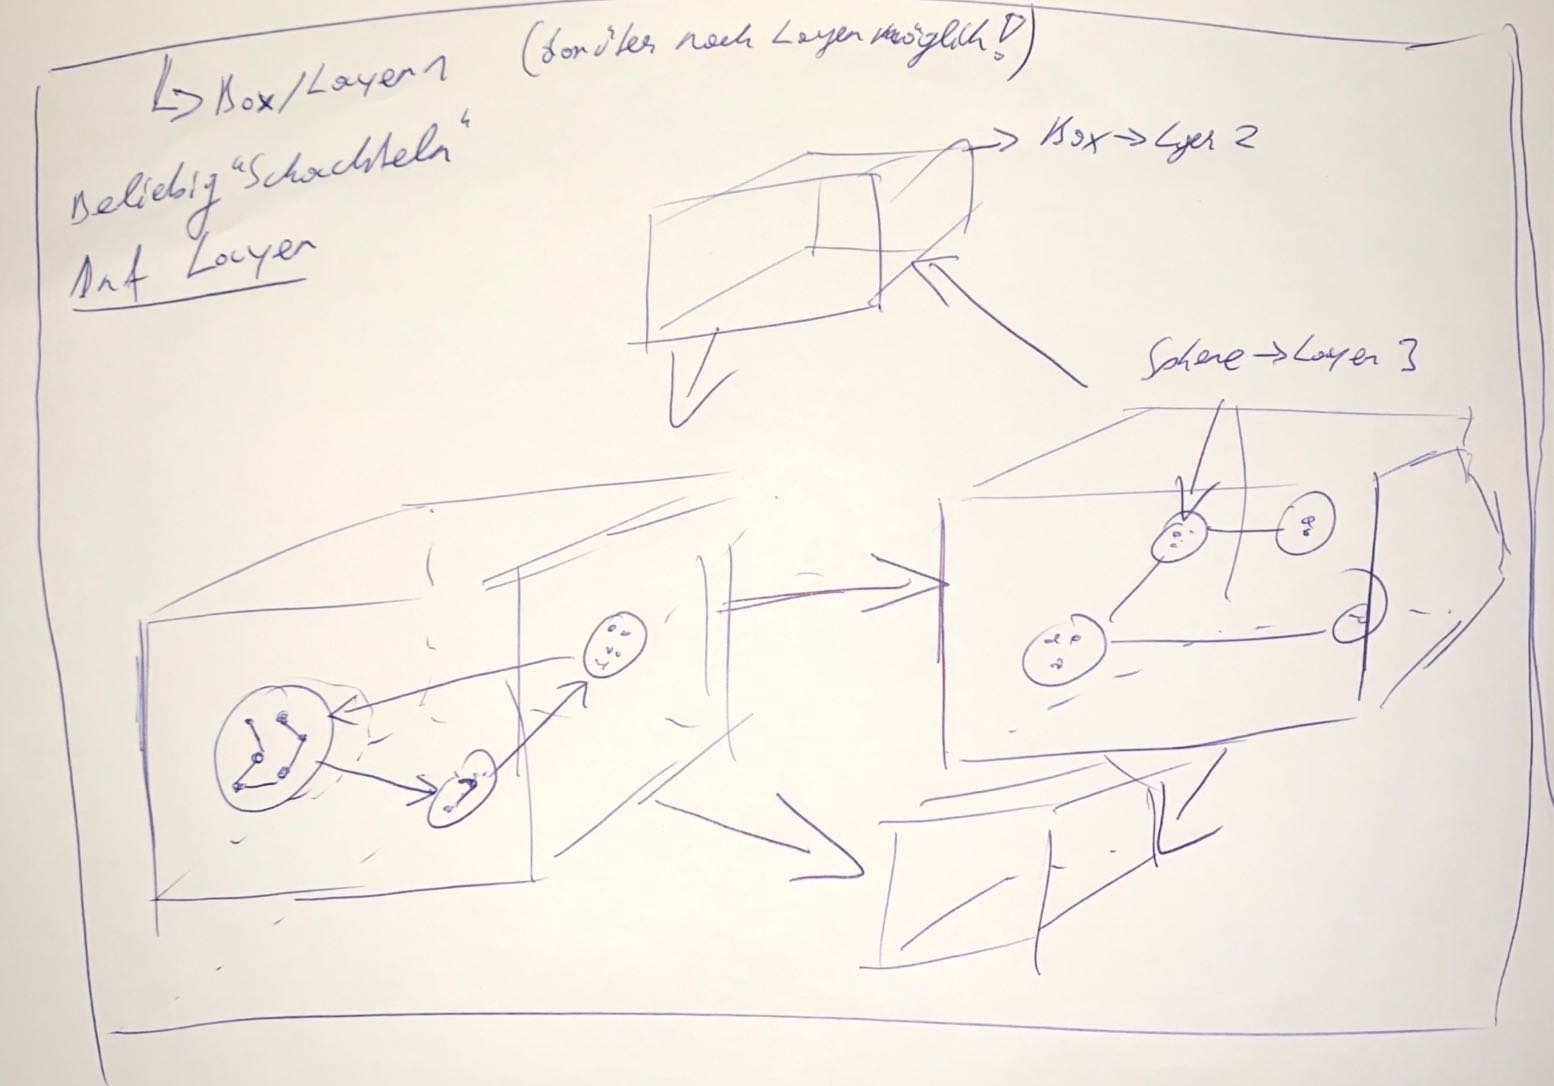
\includegraphics[width=0.5\textwidth]{chapters/graphics/concept1.jpg}

Improved concept \\
no fixed cube/(half) sphere position instead each layer calculate its own position \\
circle over boxes \\
Begin: flyspeed only, later on problem on VR \\

\section{Position of Nodes}

Independent per layer / sub-graph inside parent node \\
use of existing implemented and already good tested(prevents overlapping, good distribution, ...) forces (collision, link, manyBody, ...) \\
use of own forces to place sub-graphs inside parent graphs \\
adjustable force strengths \\
Node size grow with number of child nodes \\
\\
two possible solutions: web-worker vs live \\

\section{Usage of different Visual Features}

Position \\
linkWidth \\
linkColor \\
linkDirection \\ 
currentLayer on Controller Overlay \\ 

\section{Graph Exploration}

\subsection{Overview Layout}
Orbital Camera

\subsection{Detail Layout}
Free Fly Camera \\
change FlySpeed based on current node the camera is located. As deeper the layer as slower the flyspeed \\
Problem experiments showed this does not work well in VR --> manual / automated scaling. \\

flyToNode \\
flyToParentLayer \\

\subsection{Visibility of the Visualization}
\subsubsection{Nodes / Layers}
wireframe
\subsubsection{Links}
lockLinks

\section{Interaction}
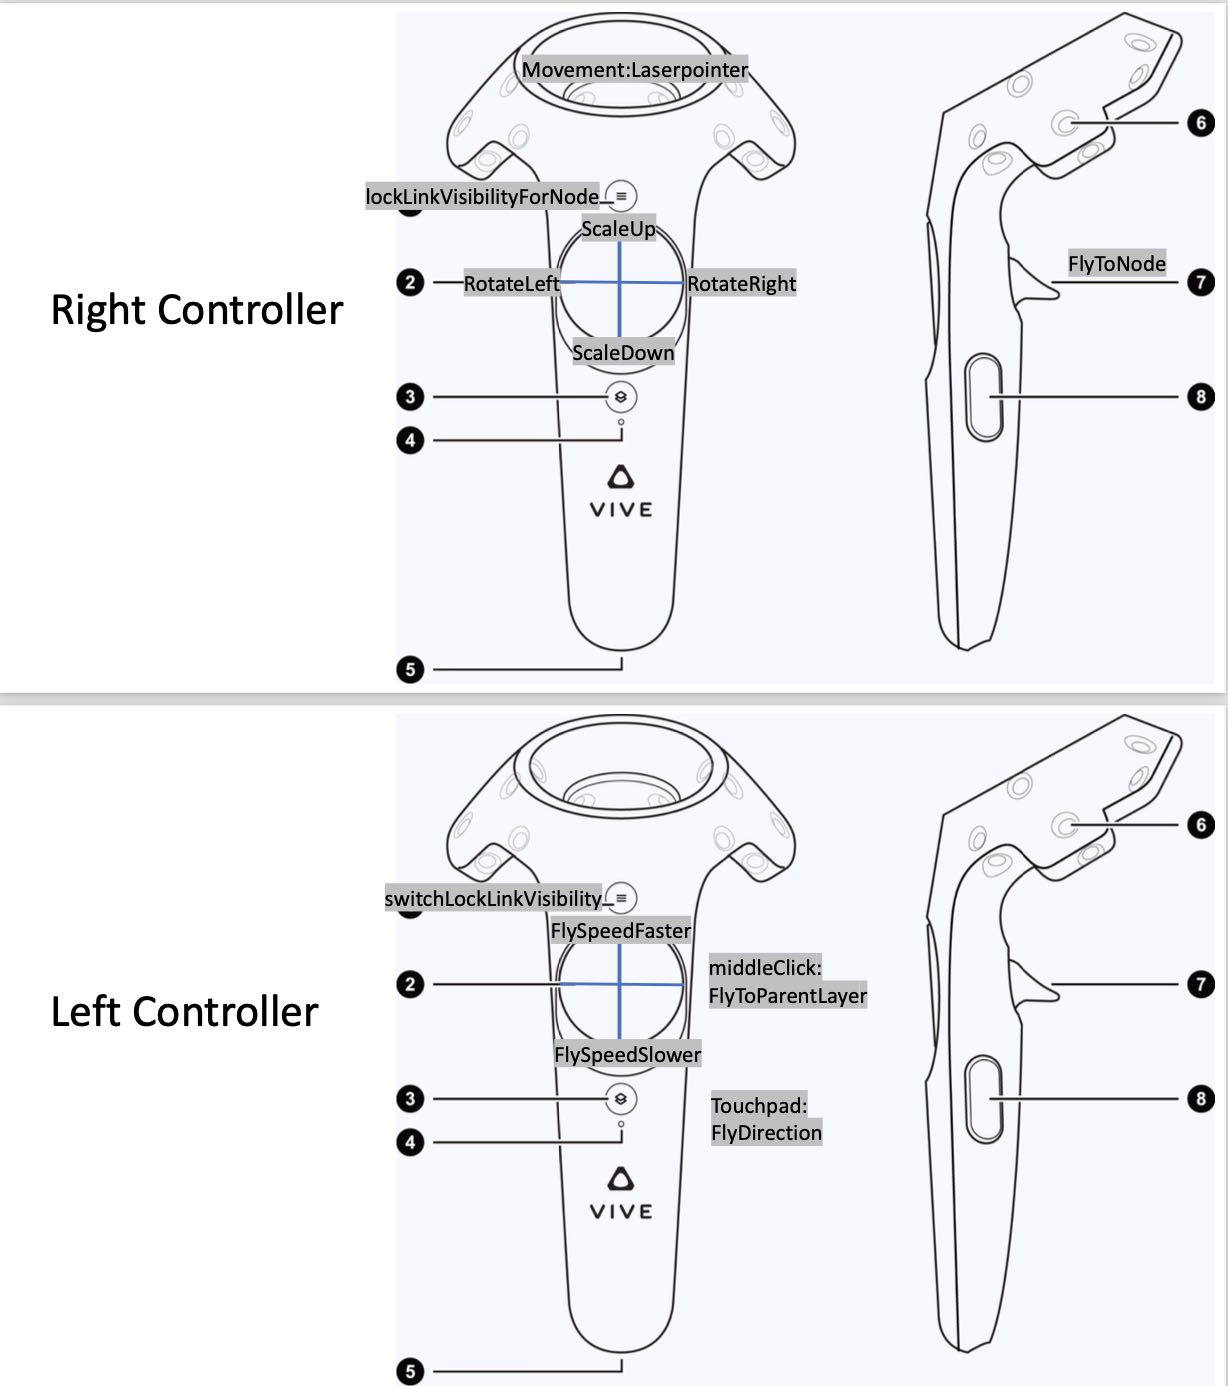
\includegraphics[width=0.5\textwidth]{chapters/graphics/controllerMapping.jpg}
